\section{Бэйзлайны}

\subsection{Задача безградиентной оптимизации}

\begin{definition}
\emph{Мета-эвристикой} (metaheuristic) называется метод black-box оптимизации
$$J(\theta) \to \max_{\theta \in \Theta}$$
со \emph{стохастическим оракулом нулевого порядка} (stochastic zeroth-order oracle), то есть возможностью для каждой точки $\theta \in \Theta$ получить несмещённую оценку $\hat{J} \HM\approx J(\theta)$.
\end{definition}

Такие методы также называются \emph{безградиентными} (gradient-free), поскольку не используют градиент функции и в принципе не предполагают её дифференцируемости. Понятно, что такие методы --- <<универсальный>> инструмент (читать, <<инструмент последней надежды>>), который можно использовать для любой задачи оптимизации. В первую очередь, этот инструмент полезен, если пространство аргументов $\Theta$ нетривиально (например, графы) или если оптимизируемая функция принципиально недифференцируема, состоит из седловых точек (<<inadequate landscape>>) или есть другие препятствия для градиентной оптимизации.

Заметим, что если $\Theta$ --- конечное множество (о градиентной оптимизации тогда речи идти не может), задача сводится к следующей: надо найти тот аргумент $\theta \in \Theta$, для которого настоящее значение $J(\theta)$ максимально, при этом используя как можно меньше стохастичных оценок $\hat{J}$ оракула. Это задача многорукого бандита, которую мы обсудим отдельно в секции \ref{sec:bandistssection}. В теории мета-эвристик опция <<запросить оракул в одной и той же точке несколько раз>> в ходе алгоритма обычно не рассматривается; предполагается достаточно богатое пространство $\Theta$, для которого более прагматичной альтернативой кажется запросить значение условно в <<соседней>> точке вместо уточнения значения оракула для одной и той же.

В контексте обучения с подкреплением, чтобы свести задачу к black-box оптимизации, достаточно представить стратегию $\pi_\theta(a \HM\mid s)$ в параметрическом семействе с параметрами $\theta \HM\in \Theta$. В качестве $J$, конечно, выступает наш оптимизируемый функционал \eqref{goal}
$$J(\theta) \coloneqq \E_{\Traj \sim \pi_\theta} R(\Traj) \to \max_{\theta},$$
а в качестве $\hat{J}$ --- его Монте-Карло оценка:
$$\hat{J}(\theta) \coloneqq \frac{1}{B}\sum_{i=1}^{B} R(\Traj_i), \quad \Traj_i \sim \pi_\theta, i \in \{1 \dots B \}$$

\begin{remark}
Если дисперсия оценки достаточно высока (число сэмплов $B$ недостаточно велико), почти все далее рассматриваемые алгоритмы сломаются (будут выживать <<везучие>>, а не <<сильнейшие>>). Поэтому может оказаться крайне существенным использовать $B > 1$, даже если $\pi_\theta$ --- семейство детерминированных стратегий.
\end{remark}

Будем проникаться местной терминологией:
\begin{definition}
Точку $\theta$, в которой алгоритм оптимизации запрашивает значение оракула, будем называть \emph{особью} (individuals, particles), а само значение $\hat{J}(\theta)$ для данной особи --- её \emph{оценкой} или \emph{приспособленностью} (fitness).
\end{definition}

В силу гигантского разнообразия мета-эвристик (от \href{https://en.wikipedia.org/wiki/List_of_metaphor-based_metaheuristics}{метода светлячков до колоний императорских пингвинов}) на полноту дальнейшее изложение, конечно же, не претендует, и стоит воспринимать рассуждение как попытку структурировать мотивации некоторых из основных идей. В частности, нас в первую очередь будут интересовать алгоритмы, в той или иной степени успешно применявшиеся в RL.

\subsection{Случайный поиск}

\emph{Случайный поиск} (random search) --- метод оптимизации и самый простой пример мета-эвристики.

\begin{definition}
Распределение $q(\theta)$ в пространстве $\Theta$ будем называть \emph{стратегией перебора}.
\end{definition}

Случайный поиск сводится к сэмплированию из стратегии перебора особей $\theta_k \HM\sim q(\theta)$ ($k \HM\in \{0, 1, 2 \dots \}$), после чего в качестве результата выдаётся особь с наилучшей оценкой.

\begin{example}[Случайный поиск]
\begin{center}
    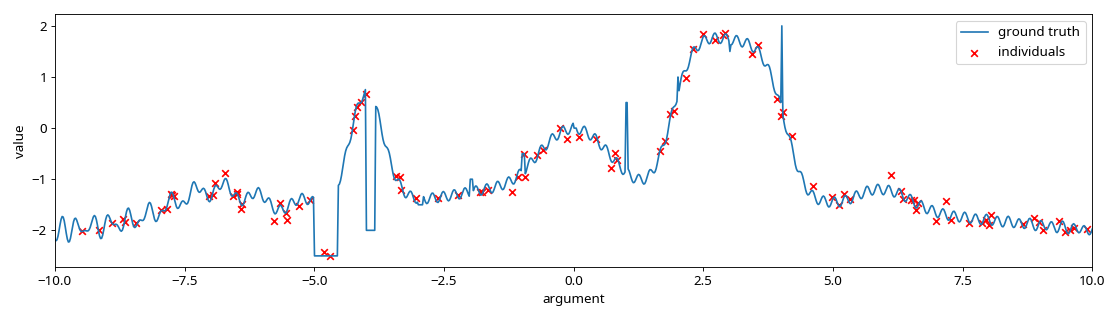
\includegraphics[width=\textwidth]{Images/randomsearch.png}
\end{center}
\end{example}

Забавно, что случайный поиск --- метод глобальной оптимизации: если $\forall \theta \HM\in \Theta \colon q(\theta) \HM> 0$, после достаточного числа итераций метод найдёт сколь угодно близкое к глобальному оптимуму решение\footnote{с оговоркой, что метод сможет понять, что нашёл оптимум, для чего придётся предположить некоторые условия регулярности для $J(\theta)$; понятно, что функцию <<иголка в стоге сена>> (needle in a haystack)
$$J(\theta) = \begin{cases}0 & \theta \neq \theta^* \\ 1 & \theta = \theta^*\end{cases}$$ никакой метод оптимизации в $\Theta \equiv \R$ не прооптимизирует.}. Есть ещё один парадокс грубого перебора: если в наличии есть неограниченное число серверов, то возможно запустить на каждом вычисление приспособленности одной особи, и за время одного вычисления провести <<глобальную>> оптимизацию.

Идея случайного поиска, на самом деле, вводит основные понятия мета-эвристик. Нам придётся так или иначе запросить у оракула приспособленности некоторого набора особей и так или иначе в итоге отобрать лучший. Для имитации умности происходящего введём весёлую нотацию.

\newcommand{\Pop}{\mathscr{P}}
\begin{definition}
Набор особей $\Pop \coloneqq \left( \theta_i \mid i \in \{1, 2 \dots N\} \right) $ называется \emph{популяцией} (population) размера $N$.
\end{definition}

\begin{definition}
Запрос оракула для всех особей популяции называется \emph{оцениванием} (evaluation) популяции:
$$\hat{J}(\Pop) \coloneqq \left( \hat{J}(\theta_i) \Bigm| i \in \{1, 2 \dots N\} \right)$$
\end{definition}

\newcommand{\Sel}{\mathrm{select}}
\begin{definition}
Процедурой \emph{отбора} (selection) называется выбор (возможно, случайный, возможно, с повторами) $M$ особей из популяции. Формально, это распределение $\Sel(\Pop^+ \mid \Pop, \hat{J}(\Pop))$, такое что $\forall \theta \in \Pop^+ \colon \theta \in \Pop$ с вероятностью 1.
\end{definition}

\newcommand{\Seltop}{\Sel^{\mathop{top}}}
\begin{definition}
\emph{Жадный} (greedy) отбор $\Seltop_M$ --- выбор топ-$M$ самых приспособленных особей.
\end{definition}

Жадный отбор плох тем, что у нас нет гарантий, что мы на самом деле выбираем наилучшую точку из рассмотренных --- наши оценки $\hat{J}$ могут быть неточны, и наилучшей на самом деле может оказаться особь с не самой высокой приспособленностью. В частности поэтому могут понадобиться альтернативы жадного отбора.

\begin{example}[Пропорциональный отбор]
Зададимся некоторым распределением на особях популяции, которые сэмплирует особь тем чаще, тем выше её приспособленность. Например:
$$p(\theta) \propto \exp{\hat{J}(\theta)}$$
Для отбора $M$ особей засэмплируем (обычно с возвращением) из этого распределения $M$ раз.
\end{example}

\begin{exampleBox}[label=ex:tournir]{Турнирный отбор}
Для отбора $M$ особей $M$ раз повторяется следующая процедура: случайно выбираются $K$ особей популяции (из равномерного распределения) и отбирается та из них, чья приспособленность выше. Число $K$ называется \emph{размером турнира} и регулирует вероятность плохо приспособленной особи быть отобранной.
\end{exampleBox}

Одна и та же особь в ходе отбора может быть выбрана несколько раз: это можно читать как <<особи повезло оставить больше потомства>>\footnote{С точки зрения эволюционной теории, критерием оптимизации для особи является исключительно преумножение количества своих генов за счёт размножения. Отбор --- не столько про <<выживание сильнейших>>, сколько про количество успешных передач генов потомкам.}.

Итак, случайный поиск можно переформулировать на языке мета-эвристик так: сгенерировать из данной стратегии перебора популяцию заданного размера $N$ и отобрать из неё 1 особь жадно.

\subsection{Hill Climbing}

Процедура отбора позволяет только <<сокращать>> разнообразие популяции. Хочется как-то обусловить процесс генерации новых кандидатов на уже имеющуюся информацию (которая состоит только из особей и их приспособленностей). Мотивация введения мутаций в том, что даже в сложных пространствах $\Theta$ зачастую можно что-то <<поделать>> с точкой $\theta$ так, чтобы она превратилась в другую точку $\hat{\theta}$.

\newcommand{\mut}{\mathfrak{m}}
\newcommand{\Mut}{\mathfrak{M}}
\begin{definition}
\emph{Мутацией} (mutation) называется распределение $\mut(\hat{\theta} \HM\mid \theta)$, где $\theta$ называется \emph{родителем} (parent), $\hat{\theta}$ --- \emph{потомком} (child).
\end{definition}

\begin{exampleBox}[label=ex:graph_mutation]{}
Пусть $\Theta$ --- множество путей обхода вершин некоторого графа. Такое пространство аргументов возникает во многих комбинаторных задачах (таких как \href{https://ru.wikipedia.org/wiki/Задача_коммивояжёра}{задача коммивояжёра}). Пусть $\theta \in \Theta$ --- некоторый путь обхода, то есть упорядоченное множество вершин графа. Мутацией может выступать выбор случайных двух вершин и смена их местами в порядке обхода (например, обходили пять вершин графа в порядке (4, 3, 1, 5, 2), а после мутации - в порядке (4, 2, 1, 5, 3)). 
\end{exampleBox}

Рассмотрим простейший способ использования мутации. На $k$-ом шаге алгоритма будем генерировать $N$ потомков особи $\theta_k$ при помощи мутации и отбирать из них жадно особь $\theta_{k+1}$. Очень похоже на градиентный подъём: мы сэмплим несколько точек вокруг себя и идём туда, где значение функции максимально. Поэтому отчасти можно считать, что Hill Climbing с большим $N$ --- локальная оптимизация: мы не можем взять наилучшее направление изменения $\theta$ из, например, градиентов, но можем поискать хорошее направление, условно, случайным перебором.

\begin{example}[Hill Climbing]
\begin{center}
\animategraphics[controls, width=\linewidth]{1}{Images/HC/hill_climbing-}{0}{9}
\end{center}
\end{example}

Что получается: если мутация такова, что $\forall \theta, \hat{\theta} \colon \mut(\hat{\theta} \HM\mid \theta) \HM> 0$, остаются гарантии оказаться в любой точке пространства, и алгоритм остаётся методом глобальной оптимизации. При этом, мутация может быть устроена так, что вероятность оказаться <<неподалёку>> от родителя выше, чем в остальной области пространства. 

\begin{example}
В предыдущем примере \ref{ex:graph_mutation} мутация не удовлетворяла свойству $\forall \theta, \hat{\theta} \colon \mut(\hat{\theta} \HM\mid \theta) \HM> 0$: из текущего пути обхода мы могли получить только очень похожий. Применение мета-эвристик к такой мутации чревато скорым застреванием в локальном оптимуме: мы можем попасть в точку, применение мутации к которой с вероятностью один даёт ещё менее приспособленные особи. Чтобы полечить это, создадим другую мутацию: засэмплируем натуральное $n$ из \href{https://ru.wikipedia.org/wiki/Распределение_Пуассона}{распределения Пуассона} или из $p(n) = \frac{1}{2^n}$ и применим такое количество мутаций вида <<сменить две вершины местами>>. Так мы гарантируем, что с небольшой вероятностью мы сможем мутировать в произвольную точку пространства аргументов.
\end{example}

Понятно, что если мутация генерирует очень непохожие на родителя особи, алгоритм схлопывается примерно в случайный поиск. И понятно, что если мутация, наоборот, с огромной вероятностью генерирует очень близкие к родителю особи, алгоритм, помимо того, что будет сходиться медленно, будет сильно надолго застревать в локальных оптимумах. Возникает trade-off между \emph{использованием} (exploitation) и \emph{исследованием} (exploration): баланс между выбором уже известных хороших точек и поиском новых <<вдали>>; изучением окрестностей найденных локальных оптимумов и поиском новых. 

\begin{exampleBox}[label=ex:gaussianmutation]{}
Если $\Theta \HM\equiv \R^h$, то типичным выбором мутации является $\mut(\hat{\theta} \HM\mid \theta) \HM\coloneqq \N(\theta, \sigma^2I_{h \times h})$, где $\sigma \HM> 0$ --- гиперпараметр, и, чем ближе $\sigma$ к нулю, тем <<ближе>> к родителю потомки.
\end{exampleBox}

\begin{remark}
Возникает вопрос: а как подбирать гиперпараметры мета-эвристик, тоже мета-эвристикой? Любопытный ответ --- \emph{самоадаптирующиеся параметры} (self-adaptive mutations). Параметры мутации кодируются в пространстве аргументов $\Theta$; то есть одна из координат каждого $\theta \in \Theta$ и отвечает за, например, дисперсию $\sigma$ в добавляемом шуме из нормального распределения. Появляется надежда, что мета-эвристика <<сама подберёт себе хорошие гиперпараметры>>.
\end{remark}

\subsection{Имитация отжига}

\emph{Имитация отжига} (simulated annealing) решает <<проблему исследования>> при помощи более умной процедуры отбора: вероятность выбрать потомка $\theta'_{k+1}$, а не остаться в родительской точке $\theta_k$, вводится так:
$$\Sel \left( \theta_{k+1} = \theta'_{k+1} \right) \coloneqq \min \left(1, \exp{\frac{\hat{J}(\theta'_{k+1}) - \hat{J}(\theta_k)}{\tau_k}} \right)$$
где $\tau_k \HM> 0$ --- \emph{температура}, гиперпараметр, зависящий от номера итерации. Иными словами, если новая точка более приспособлена, то мы принимаем новую точку $\theta'_{k+1}$ с вероятностью 1; если же новая точка менее приспособлена, мы не выкидываем её, а переходим в неё с некоторой вероятностью. Эта вероятность тем ближе к единице, чем <<похожее>> значения оракула, и температура регулирует понятие похожести между скалярами относительно масштаба оптимизируемой функции $J$.

Наша цепочка $\theta_0, \theta_1, \theta_2 \dots$ задаёт марковскую цепь: мы генерируем каждую следующую особь на основе только предыдущей, используя некоторое стохастичное правило перехода. Теория марковских цепей говорит, что может существовать \emph{стационарное распределение} (stationary distribution): распределение, из которого приходят $\theta_k$, при стремлении $k \to \infty$ всё ближе к некоторому $p(\theta)$, которое определяется лишь нашей функцией переходов и не зависит от инициализации $\theta_0$.

\begin{theorem}[Алгоритм Метрополиса-Гастингса]
Пусть в пространстве $\Theta$ задано распределение $p(\theta)$ и распределение $q(\hat{\theta} \HM\mid \theta)$, удовлетворяющее $\forall \hat{\theta}, \theta \colon q(\hat{\theta} \HM\mid \theta) > 0$. Пусть строится цепочка $\theta_0, \theta_1, \theta_2 \dots$ по следующему правилу: генерируется $\theta'_{k+1} \HM\sim q(\theta'_{k+1} \HM\mid \theta_k)$, после чего с вероятностью
$$\min \left( 1, \frac{p(\theta'_{k+1})}{p(\theta_{k})}\frac{q(\theta_k \HM\mid \theta'_{k+1})}{q(\theta'_{k+1} \HM\mid \theta_{k})} \right)$$
$\theta_{k+1}$ полагается равным $\theta'_{k+1}$, а иначе $\theta_{k+1} \coloneqq \theta_k$.
Тогда для любого $\theta_0$:
$$\lim_{k \to \infty} p(\theta_k) = p(\theta)$$
\begin{proof}[Без доказательства]
\end{proof}
\end{theorem}

\begin{proposition}
Пусть оракул точный, то есть $\hat{J}(\theta) \equiv J(\theta)$, а мутация удовлетворяет
$$\forall \theta, \hat{\theta} \colon \mut(\hat{\theta} \HM\mid \theta) = \mut(\theta \HM\mid \hat{\theta}) > 0.$$
Тогда, если температура $\tau$ не зависит от итерации, для любой инициализации $\theta_0$ алгоритм имитации отжига строит марковскую цепь со следующим стационарным распределением:
$$\lim_{k \to \infty} p(\theta_k) \propto \exp \frac{J(\theta_k)}{\tau}$$
\end{proposition}

Алгоритм Метрополиса даёт, вообще говоря, <<гарантии сходимости>> для имитации отжига: то, что через достаточно большое количество итераций мы получим сэмпл из распределения $\exp \frac{J(\theta_k)}{\tau}$, нас, в общем-то, устраивает: если температура достаточно мала, это распределение очень похоже на вырожденное в точке максимального значения оптимизируемой функции. Однако, малая температура уменьшает долю исследований в алгоритме, и тогда алгоритм вырождается в наивный поиск при помощи мутации. Поэтому на практике температуру снижают постепенно; подобный \emph{отжиг} (annealing) часто применяется для увеличения доли исследований в начале работы алгоритма и уменьшения случайных блужданий в конце.

\begin{example}[Имитация отжига]
\begin{center}
\animategraphics[controls, width=\linewidth]{1}{Images/SA/simulated_annealing-}{0}{9}
\end{center}
\end{example}

\begin{remark}
Если в операторе мутации есть параметр, отвечающий за <<силу мутаций>>, например дисперсия $\sigma$ гауссовского шума в примере \ref{ex:gaussianmutation}, а то есть тоже связанный с балансом исследования-использования, его аналогично можно подвергнуть отжигу: в начале алгоритма его значение выставляется достаточно большим, после чего по некоторому расписанию уменьшается с ходом алгоритма.
\end{remark}

\subsection{Эволюционные алгоритмы}

Hill Climbing --- эвристика с <<одним состоянием>>: есть какая-то одна текущая основная особь-кандидат, на основе которой и только которой составляется следующая особь-кандидат. Нам, вообще говоря, на очередном шаге нам доступна вся история проверенных точек. Первый вариант --- построить суррогат-приближение $\hat{J}(\theta)$, которую легко можно прооптимизировать и найти так следующего кандидата (к нему относятся, например, алгоритмы на основе \href{https://distill.pub/2020/bayesian-optimization/}{гауссовских процессов}), но этот вариант не сработает в сложных пространствах $\Theta$. Второй вариант --- перейти к <<эвристикам с $N$ состояниями>>, то есть использовать последние $N$ проверенных особей для порождения новых кандидатов.

\begin{definition}
\emph{Эволюционный} (evolutionary) алгоритм строит последовательность популяций $\Pop_1, \Pop_2 \dots$, на $k$-ом шаге строя очередное \emph{поколение} (generation) на основе предыдущего.
\end{definition}

Практически все мета-эвристики сводятся к эволюционным алгоритмам. При этом заметим, что, пока единственным инструментом <<генерации>> новых особей выступает мутация, алгоритмы различаются только процедурой отбора. Таким образом, в алгоритме всегда поддерживается текущая популяция из $N$ особей (первая популяция генерируется из некоторой стратегии перебора $q(\theta)$), из них отбирается $N$ особей (отбор может выбирать одну особь несколько раз, поэтому этот шаг нетривиален), и дальше каждая отобранная особь мутируется. Эвристика \emph{элитизма} (elitism) предлагает некоторые из отобранных особей не мутировать, и оставить для следующей популяции; это позволяет уменьшить шансы популяции <<потерять>> найденную область хороших значений функции, но увеличивает шансы застревания в локальном оптимуме. При элитизме для каждой особи хранится её \emph{возраст} (age) --- число популяций, через которые особь прошла без мутаций; далее этот возраст влияет на отбор, например, выкидывая все особи старше определённого возраста. Далее будем рассматривать алгоритмы без элитизма.

Придумаем простейший эволюционный алгоритм. Любой алгоритм локальной оптимизации (градиентный спуск или Hill Climbing), результат работы которого зависит от начального приближения $\theta_0 \sim q(\theta)$, можно <<заменить>> на метод глобальной оптимизации, запустив на каждом условном сервере по <<\emph{потоку}>> (thread) со своим начальным $\theta_0$. Время работы алгоритма не изменится (считая, конечно, что сервера работают параллельно), а обнаружение неограниченного числа локальных оптимумов с ненулевым шансом найти любой гарантирует нахождение глобального. Набор из текущих состояний всех потоков можно считать текущей популяцией.

При этом, любая процедура отбора позволит потокам <<обмениваться информацией между собой>>. Для примера рассмотрим распространённую схему \emph{$(M, K)$-эволюционной стратегии}, в которой процедура отбора заключается в том, чтобы топ-$M$ особей отобрать по $K$ раз каждую (дать каждой особи из топа породить $K$ детей). Иными словами, мы параллельно ведём $M$ Hill Climbing-ов, в каждом из которых для одного шага генерируется $K$ потомков; если число потоков $M = 1$, алгоритм вырождается в обычный Hill Climbing. Порождённые $N = MK$ особей образуют текущую популяцию алгоритма. Среди них отбирается $M$ лучших особей, которые могут как угодно распределиться по потокам. Получится, что некоторые потоки, которые не нашли хороших областей $\Theta$, будут прерваны, а хорошие получат возможность сгенерировать больше потомков и как бы <<размножаться>> на несколько процессов. 

\begin{algorithm}{$(M, K)$-эволюционная стратегия}
\textbf{Дано:} оракул $\hat{J}(\theta)$ \\
\textbf{Гиперпараметры:} $\mut(\hat{\theta} \mid \theta)$ --- мутация, $q(\theta)$ --- стратегия перебора, $M$ --- число потоков, $K$ --- число сэмплов на поток

\vspace{0.3cm}
Инициализируем $\Pop_0 \coloneqq \left( \theta_i \sim q(\theta) \mid i \in \{1, 2, \dots , MK \} \right)$ \\
\textbf{На $k$-ом шаге:}
\begin{enumerate}
    \item проводим жадный отбор: $\Pop^{+}_k \coloneqq \Seltop_M(\Pop_k, \hat{J}(\Pop_k))$
    \item размножаем: $\Pop_{k+1} \coloneqq \left( \hat{\theta}_i \sim \mut(\hat{\theta} \mid \theta) \mid \theta \in \Pop^{+}_k, i \in \{1, 2, \dots , K\} \right)$
\end{enumerate}
\end{algorithm}

\begin{example}[(4, 5)-эволюционная стратегия]
\begin{center}
\animategraphics[controls, width=\linewidth]{1}{Images/MS_ES/ms_es-}{0}{8}
\end{center}
\end{example}

\subsection{Weight Agnostic Neural Networks (WANN)}

Поскольку мета-эвристики --- универсальный метод оптимизации, они могут применяться к нейронным сетям. Такой подход даёт такие преимущества, как возможность использовать дискретные веса или недопустимые для градиентной оптимизации функции активации вроде функции Хевисайда. 

Особенностью \emph{нейроэволюции} (neuroevolution) является возможность искать топологию сети вместе со значениями самих весов: для этого достаточно предложить некоторый оператор мутации. Рассмотрим распространённый пример: пусть дана некоторая нейросеть с произвольной топологией\footnote{на заре нейросетевого подхода разумность использования полносвязных слоёв была под вопросом. Считаем, что нейрон принимает несколько входов, домножает каждый вход на некоторый вес, складывает и применяет функцию активации, выдавая скалярную величину. Выход нейрона отправляется некоторым из других нейронов на вход; понятие <<слоёв>> обычно не вводится.} и некоторыми весами. Для весов процедуру мутирования можно взять стандартную (добавление шума с заданной дисперсией; дополнительно можно для каждого веса сэмплировать бинарную величину, будет ли данный вес мутировать). Далее случайно выбирается, будет ли проходить мутация архитектуры (топологии) сети, и если да, то какого типа (обычно рассматривается несколько типов мутации).

\begin{exampleBox}[label=ex:wannmutations]{Топологические мутации нейросети}
Распространён набор из трёх видов топологических мутаций: добавление связи, добавление нейрона и смена функции активации. 

\begin{wrapfigure}{r}{0.3\textwidth}
\centering
\vspace{-0.5cm}
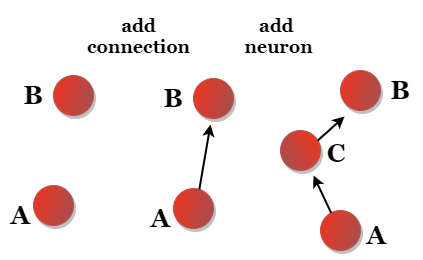
\includegraphics[width=0.3\textwidth]{Images/topologymutation.png}
\vspace{-1cm}
\end{wrapfigure}

Добавление связи означает, что случайно выбираются два ранее не соединённых связью нейрона и выход одного подаётся добавляется к входу в другой (вес инициализируется случайно). Какой из двух нейронов является входом, а какой --- выходом, однозначно определяется требованием ацикличности к вычислительному графу. Под добавлением нейрона понимается именно разбиение уже имеющейся связи: имевшаяся связь A--B, где A, B --- нейроны, выключается, и появляются связи A--C и C--B, где C --- новый нейрон. Новые нейроны необходимо добавлять именно так, чтобы они сразу же участвовали в вычислительном процессе. Смена функции активации меняет функцию активацию в случайном нейроне на произвольную из набора.
\end{exampleBox}

\begin{remark}
Заметим, что операторе мутации из примера \ref{ex:wannmutations} отсутствуют шансы на уменьшение числа связей. Эволюционный процесс с таким оператором мутации будет рассматривать пространство $\Theta$ нейросетей с различными топологиями от <<более простых>> архитектур к <<более сложным>>. В частности поэтому рекомендуется изначально алгоритм инициализировать <<пустой>> топологией: между входами и выходами связей нет, а появляться они будут в ходе постепенных мутаций. Похоже, что к такой эвристике привёл эмпирический опыт, и введение мутаций, удаляющих часть архитектуры, не приводило к особым успехам; результатом работы нейроэволюционного алгоритма типично является крайне минимальная по современным меркам нейросеть, с довольно малым количеством связей.
\end{remark}

\emph{Weight Agnostic} сети зашли ещё дальше и, по сути, отказались от настройки весов нейросети в принципе, ограничившись только поиском топологии. Алгоритм WANN основан на $(M, K)$-эволюционной стратегии с оператором мутации из рассмотренного примера \ref{ex:wannmutations}. Единственным изменением является процедура отбора. Для данной топологии оракул запускается шесть раз. В каждом запуске всем весам сети присваивается одно и то же значение (авторы использовали значения $[-2, -1, -0.5, 0.5, 1, 2]$). Рассматривается три критерия приспособленности особи: среднее из шести значение $\hat{J}$, максимальное из шести значение $\hat{J}$ и число связей. Эти три критерия не смешиваются со скалярными гиперпараметрами, вместо этого проводится турнирный отбор (пример \ref{ex:tournir}): из популяции выбираются два кандидата, выбирается случайный критерий, и выживает сильнейший по данному критерию. Так отбирается $M$ особей, которые и порождают $K$ потомков каждый.

\subsection{Видовая специализация}\label{specieisidea}

Возникает простой вопрос к $(M, K)$-эволюционной стратегии: а не случится ли такого, что он схлопнется к Hill Climbing-у, если в очередной популяции среди топ-$M$ останутся только дети одного и того же родителя? Получится, что, хоть мы и исходили из идеи исследовать параллельно много локальных оптимумов, жадный отбор может убить все потоки, кроме одного, и <<область пространства аргументов>>, покрываемая текущей популяцией, <<схлопнется>>.

Для борьбы с этим эффектом в мета-эвристиках рассматривают методы \emph{защиты инноваций} (innovation protection). Если для получения новых хороших свойств необходимо сделать <<несколько>> шагов эволюции, то мы каким-то образом помогаем выживать особям, оказавшихся в не исследующихся местах пространства $\Theta$. Самый простой способ --- использование более <<мягких>> процедур отбора, когда у неприспособленной особи есть небольшой шанс выжить. Более интеллектуально было бы как-то оценить, насколько <<новой>> является область пространства аргументов, в которой оказалась особь, и дать ей больше шансов выжить, если алгоритм эту область ещё не рассматривал: ведь проблема мягких процедур отбора, очевидно, в том, что выживают слабые особи и там, где функция уже была в достаточной степени исследована.

Рассмотрим общую идею \emph{видов} (species). Допустим, мы сможем в $\Theta$ придумать метрику (или хоть сколько-то функцию близости) $\rho(\theta_1, \theta_2)$ и на её основе разбить все особи популяции $\Pop$ на непересекающиеся множества --- <<виды>>. Процесс разбиения, что важно, не обязан удовлетворять каким-то особым свойствам и может быть стохастичным, в том числе чтобы быть дешёвым. 

\begin{exampleBox}[label=ex:species]{Процедура разделения на виды}
Изначально множество видов пусто. На очередном шаге берём очередную особь из $\Pop$ и в случайном порядке перебираем имеющиеся виды. Для каждого вида сэмплируем одну из ранее отнесённых к нему особей и сравниваем расстояние $\rho$ с порогом-гиперпараметром процесса: меньше порога --- относим рассматриваемую особь к этому виду и переходим к следующей особи, больше порога --- переходим к следующему виду. Если ни для одного вида проверка не прошла, особь относится к новому виду. Пересчёт видов проводится для каждой популяции заново.
\end{exampleBox}

Разделение на виды позволяет делать, например, \emph{explicit fitness sharing}: особи соревнуются только внутри своих видов. Пусть $\widetilde{\Pop} \subseteq \Pop$ --- вид, а $\hat{J}_{\mathop{mean}}(\widetilde{\Pop})$ --- среднее значение приспособленности в данном виде. Тогда на основе этих средних значений между видами проводится (в некоторой <<мягкой>> форме --- слабые виды должны выживать с достаточно высокой вероятностью) некоторый мягкий отбор; например, виду $\widetilde{\Pop}$ позволяется сгенерировать потомков пропорционально $\exp \hat{J}_{\mathop{mean}}(\widetilde{\Pop})$ с учётом того, что в сумме все виды должны породить заданное гиперпараметром число особей. Генерация необходимого числа потомков внутри каждого вида происходит уже, например, стандартным, <<агрессивным>> образом: отбирается некоторая доля топ-особей, к которым и применяется по несколько раз мутация.

Виды защищены мягким отбором и поэтому заспавнивнишеся вдали особи, образующие новый вид, будут умирать реже; при этом в скоплениях слабых особей в одном месте пройдёт жёсткий внутривидовой отбор, а сам вид получит не так много <<слотов потомства>>, и число точек сократится.

\begin{example}[Эволюция с видовой специализацией]
В данном примере текущая популяция из 20 особей разделяется на виды согласно процедуре из примера \ref{ex:species} с метрикой $\rho(\theta_1, \theta_2) = |\theta_1 - \theta_2|$ и порогом 1. Для видов считается $\hat{J}_{\mathop{mean}}(\widetilde{\Pop})$ (указан как fit в легенде), после чего при помощи сэмплирования из распределения $\propto \exp \hat{J}_{\mathop{mean}}(\widetilde{\Pop})$ 20 раз разыгрываются между видами <<слоты потомства>>. Внутри каждого вида жадно отбирается 1 особь, она и порождает разыгранное число потомков. Разбиение на виды проводится для новой полученной популяции заново.
\begin{center}
\animategraphics[controls, width=\linewidth]{1}{Images/EL_ES/el_es-}{0}{9}
\end{center}
\end{example}

\subsection{Генетические алгоритмы}

До сих пор мы умели создавать новые особи только при помощи мутации. В генетических алгоритмах дополнительно вводится этап \emph{рекомбинации} (recombination), когда новые особи можно строить на основе сразу нескольких особей, как-то <<совмещая>> свойства тех и других в надежде получить <<лучшее от двух миров>>; найти хороший оптимум между двумя локальными оптимумами. В ванильной версии генетических алгоритмов у детей по два родителя, хотя можно рассматривать и скрещивание большего числа особей:

\newcommand{\cross}{\mathfrak{c}}
\begin{definition}
\emph{Кроссинговером} (crossover) называется распределение $\cross(\hat{\theta} \HM\mid \theta_1, \theta_2)$, где $\theta_1, \theta_2$ называются \emph{родителями} (parent), $\hat{\theta}$ --- \emph{потомком} (child).
\end{definition}

\begin{example}
Для $\Theta \equiv \R^d$ или $\Theta \equiv \{0, 1\}^d$ (или их смеси) можно придумать много разных кроссинговеров; генетика подсказывает, что если элементы векторов это <<гены>>, то нужно, например, некоторые гены взять от одного родителя, а другие от другого. Некоторые гены можно \emph{сцеплять} (сцепленные гены должны быть взяты из одного родителя), или вводить порядок на генах (брать от одного родителя <<правую>> часть, от другого <<левую>>).
\end{example}

Чтобы сохранить свойство <<глобальности>> оптимизации, желательно было бы, опять же, чтобы мы могли при помощи такого инструмента порождения оказаться в любой точке пространства, т.е. $\forall \hat{\theta}, \theta_1, \theta_2 \HM\in \Theta \colon \cross(\hat{\theta} \HM\mid \theta_1, \theta_2) > 0$. Однако, для практически любых примеров кроссинговера это не так. Поэтому считается, что это требование НЕ выполняется: процедура рекомбинации, возможно, стохастична, но всегда приводит к точке <<между>> $\theta_1$ и $\theta_2$. Это означает, что, используя только кроссинговер, область, покрываемая потомством, будет уже области, покрываемой родителями: теряется исследование. Чтобы полечить это, в генетических алгоритмах всё равно остаётся этап применения мутации.

\begin{algorithm}[label=geneticsearch]{Генетический поиск}
\textbf{Дано:} оракул $\hat{J}(\theta)$ \\
\textbf{Гиперпараметры:} $\cross(\hat{\theta} \mid \theta_1, \theta_2)$ --- кроссинговер, $\mut(\hat{\theta} \mid \theta)$ --- мутация, $\Sel(\Pop^+ \mid \Pop, \hat{J}(\Pop))$ --- процедура отбора, $q(\theta)$ --- стратегия перебора, $N$ --- размер популяции

\vspace{0.3cm}
Инициализируем $\Pop_0 \coloneqq \left( \theta_i \sim q(\theta) \mid i \in \{1, 2, \dots , N \} \right)$ \\
\textbf{На $k$-ом шаге:}
\begin{enumerate}
    \item проводим отбор: $\Pop^{+}_k \sim \Sel(\Pop^{+}_k \mid \Pop_k, \hat{J}(\Pop_k))$
    % TODO прокол
    \item проводим размножение: $\Pop_{k+1} \coloneqq \left( \theta_i \sim \cross \left( \theta \mid \theta_l, \theta_r \right) \mid \theta_l, \theta_r \in \Pop^{+}_k \right)$
    \item проводим мутирование: $\Pop_{k+1} \leftarrow \left( \hat{\theta} \sim \mut (\hat{\theta} \mid \theta) \mid \theta \in \Pop_{k+1} \right)$
\end{enumerate}
\end{algorithm}

\begin{remark}
При эволюционном обучении нейросетей, в отличие от ряда других задач, кроссинговер во многом неудобен. Нельзя взять <<половинку>> одной хорошей нейросети и присоединить к <<половинке>> другой хорошей нейросети --- каждый нейрон рассчитывает на тот набор входов, для которого он был обучен (неважно, эволюционно или градиентно). Поэтому генетические алгоритмы для нас не представляют особого интереса, по крайней мере на момент написания данного текста. 
\end{remark}

\begin{example}[Neuroevolution of Augmented Topologies (NEAT)]
Рассмотрим в качестве примера набор эвристик нейроэволюционного алгоритма NEAT, который всё-таки был основан на генетическом поиске (алг.~\ref{geneticsearch}), то есть дополнительно вводил оператор кроссинговера для нейросетей (двух произвольных топологий).

\begin{wrapfigure}{r}{0.35\textwidth}
\centering
\vspace{-0.5cm}
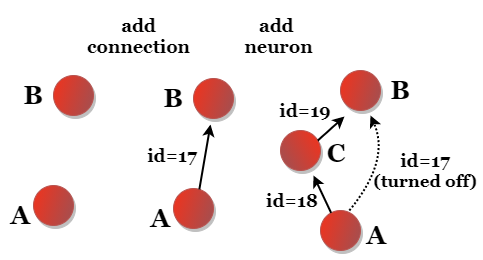
\includegraphics[width=0.35\textwidth]{Images/neatmutation.png}
\vspace{-0.7cm}
\end{wrapfigure}

В NEAT все связи всех особей, помимо веса, имеют статус <<включена-выключена>> и уникальный идентификационный номер (id), или \emph{исторический маркер} (historical marker). Связи могут появляться только в ходе мутаций (используется оператор мутации из примера \ref{ex:wannmutations}); в момент создания связи ей присваивается уникальный (в рамках всего алгоритма) id и статус <<включена>>. Наличие у двух особей связи с одним id будет означать наличие общего предка. У изначальной <<пустой>> топологии связей нет вообще. Связь может попасть в статус <<выключена>> только во время мутации вида <<добавление нейрона>>, когда имевшаяся связь A--B <<исчезает>>: то есть, соответствующий <<ген>> не удаляется из генома особи, а переходит в статус <<выключена>>. Выключенная связь означает, что у особи был предок, у которого связь была включена.

Как введение статусов и id-шников связей позволяет устраивать между разными топологиями кроссинговер? Если связь с данным id имеется у обоих скрещиваемых особей, связь сохраняется и у потомка, с весом и статусом случайного родителя. Связи, имеющиеся только у одного из родителей, будем называть \emph{непарными}; они копируются из того родителя, чья приспособленность выше (или из обоих сразу, если приспособленности одинаковые).

\begin{center}
    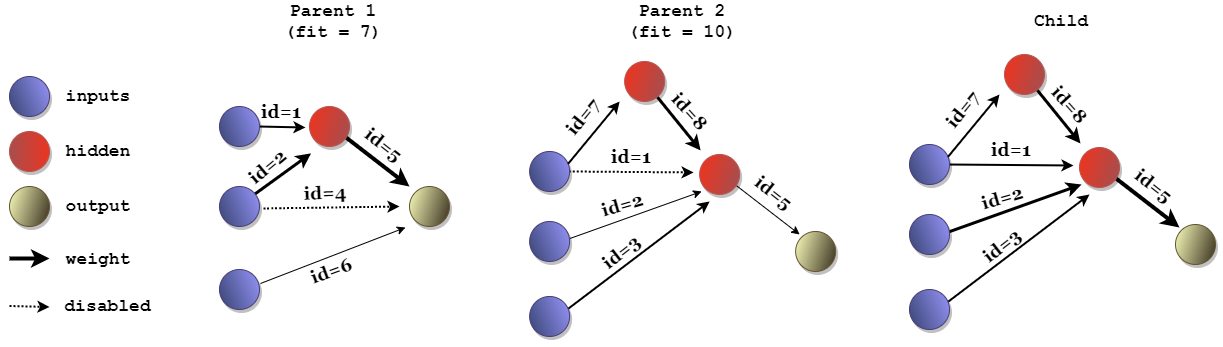
\includegraphics[width=\textwidth]{Images/neat}
\end{center}

NEAT также использует видовую специализацию (как описано в разделе \ref{specieisidea}) для процесса отбора, для чего на таких генотипах необходимо задать метрику $\rho$. Пусть $\theta_1, \theta_2$ --- две особи, $G_1, G_2$ --- количество связей у этих особей, $D$ --- число непарных связей, $w_1, w_2$ --- веса особей в парных связях. Понятно, что веса мы можем сравнить только для парных связях, и понятно, что чем больше непарных связей, тем больше должно быть расстояние. В NEAT предлагается просто объединить эти два критерия: 
$$\rho(\theta_1, \theta_2) \coloneqq \alpha_1 \frac{D}{max(G_1, G_2)} + \alpha_2 \|w_1 - w_2\|_1$$
где $\alpha_1, \alpha_2$ --- гиперпараметры. Внутри самих видов отбор жадный.

NEAT --- исторически один из первых алгоритмов, которые можно с каким-то результатом применить для RL задач без подготовленного удобного признакового описания состояний, например, изображений. Можно найти много интересных примеров применения алгоритма к простейшим задачам, с визуализацией получающейся сети (например, \href{https://www.youtube.com/watch?v=qv6UVOQ0F44}{Mario}). 

\end{example}

